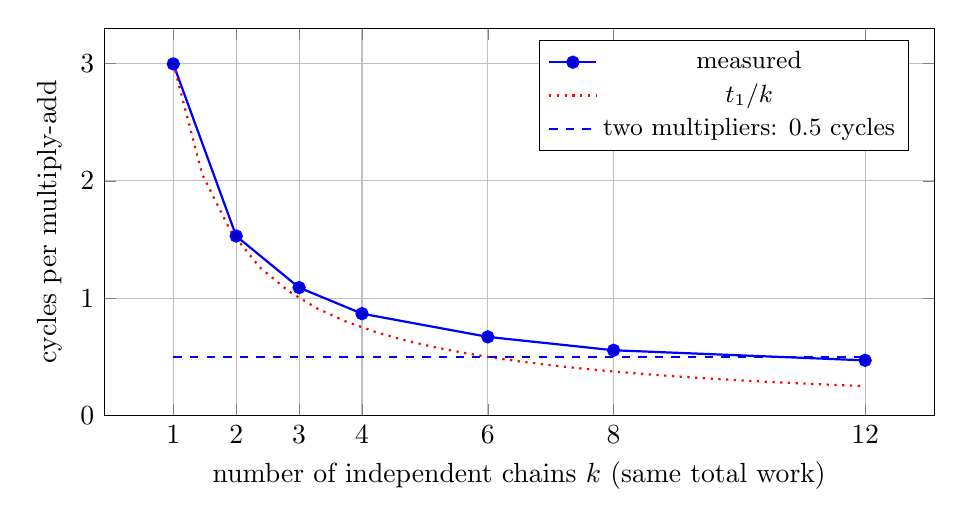
\begin{tikzpicture}
\begin{axis}[width=\textwidth, height=6.5cm, xlabel={number of independent chains $k$ (same total work)}, ylabel={cycles per multiply-add}, grid=major, ymin=0, xtick={1,2,3,4,6,8,12}, legend pos=north east, legend style={font=\small}]
\addplot+[mark=*, thick, error bars/.cd, y dir=both, y explicit] coordinates {(1,2.996) +- (0,0.003) (2,1.529) +- (0,0.002) (3,1.090) +- (0,0.001) (4,0.868) +- (0,0.015) (6,0.670) +- (0,0.002) (8,0.556) +- (0,0.002) (12,0.470) +- (0,0.001)};
\addlegendentry{measured}
\addplot[red, dotted, thick, domain=1:12] {3.00/x};
\addlegendentry{$t_1/k$}
\addplot[blue, dashed, thick, domain=1:12] {0.5};
\addlegendentry{two multipliers: 0.5 cycles}
\end{axis}
\end{tikzpicture}